In order to find the most suitable algorithm for translating a live input stream of American SLA to any other suitable SLA (sharing the same alphabet) in a real-world application, the algorithm needs to excel in two main aspects: accuracy and inference time. A third factor that may come into question here is the training time, as computational cost may accumulate when further improving the model in the future.

\subsection{The long list}\label{chapter_long}
As mentioned in chapter \ref{chapter_models} the long list contained 27 pretrained models. Due the the limited availability of computational ressources, the models on the list as per table \ref{tab:keras_models} (including all variants) were trainined in an experimental setup, to determine which models are suitable for a full training. The goal was to use these pretrained models and only train the last layer to enable the detection of SLA in sources such as webcam feeds, videos or images.

The experimental setup was trained on a consumer pc, with a 3.8 Ghz 6-core CPU, a \textit{GeForce GTX 1060} GPU and 32GB of RAM. The results mainly focus on two aspects in order to decide which models may be suitable for the full training: training time and accuracy. As shown in Fig. \ref{fig:long_list_acc} some of the models already have a high accuracy with a minified training.

\begin{figure}[h]
    \centering
    \caption{Accuracy on long list training}
	\label{fig:long_list_acc}
    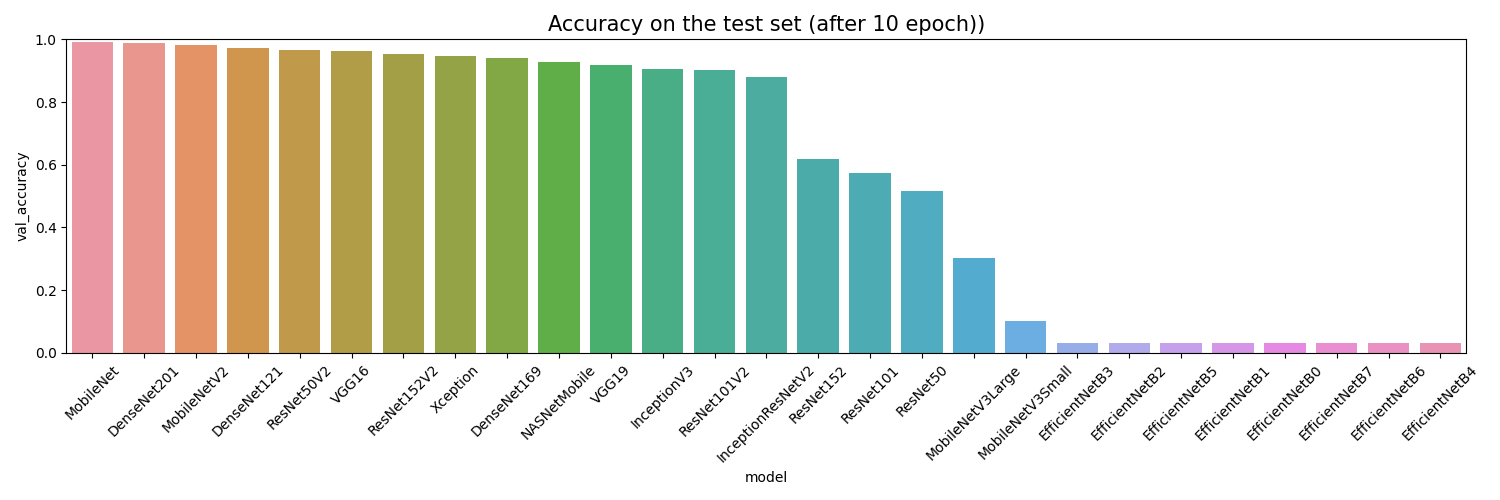
\includegraphics[width=\linewidth]{figures/long_val_accuracy.png}
\end{figure}

While models as \textit{DenseNet} seem to have good results with all variants, others like \textit{ResNet} have a high variety, accuracy ranges from ~55\% (\textit{ResNet50}) to ~98\% \textit{ResNet50V2}. The \textit{EfficientNet} with all its variants has an accuracy below 10\% and will not move forward.

\begin{figure}[h]
    \centering
    \caption{Training time on long list training}
	\label{fig:long_list_time}
    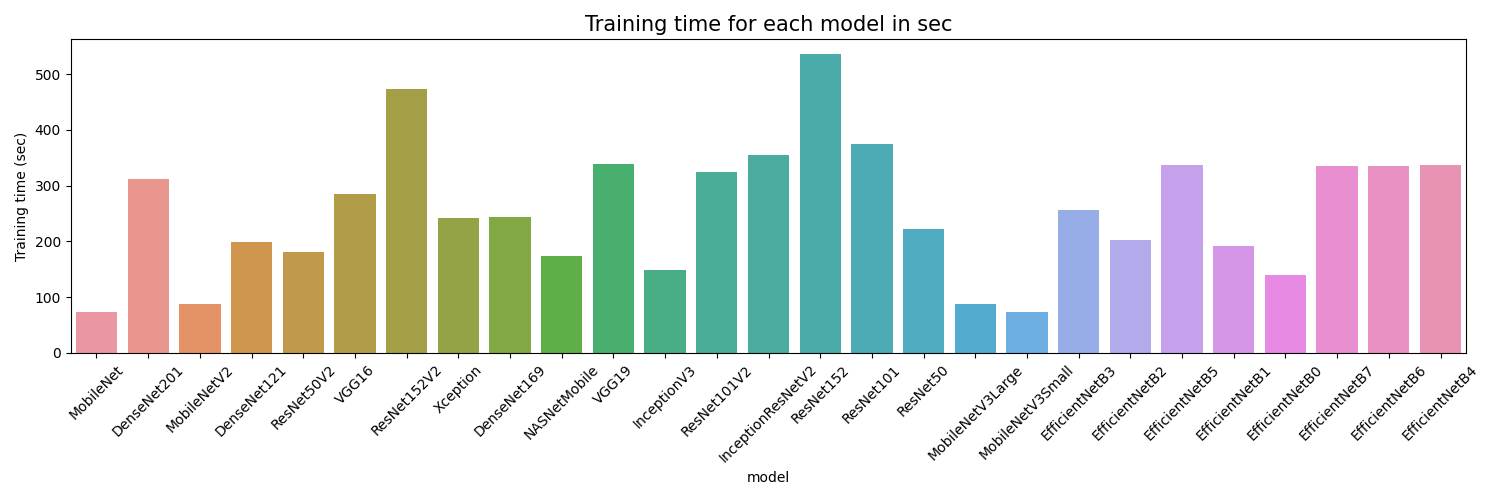
\includegraphics[width=\linewidth]{figures/long_training_time.png}
\end{figure}

Fig. \ref{fig:long_list_time} shows the time that was needed to train the models with the reduced dataset for 10 epochs without early stopping. While it shows a wide range, the times train not too long at all. Therefore, the training time will not be the main factor for deciding which model we should move forward with.

When deploying the model in a real-time environment, such as a live detection via a webcam another factor comes into play: the inference time. As described in chapter \ref{chapter_models}, the models differ fundamentally in their architecture. At this point, it is uncertain how the architecural structure will affect the inference time of a fully trained model. Therefore we decided to move forward with the best performing model from each architecture described in chapters \ref{chapter_vgg16} to \ref{chapter_xception}. In addition to the top 5 models, we decided to add \textit{MobileNetV2} as well, as it seemed interesting why the newer version of the model did perform worse than the old one. Table \ref{tab:results:long} contains all models that will be used for a full training.

\begin{table}[th]
    \caption{Short List candidates}
    \label{tab:results:long}
    \centering
    \begin{tabular}{lll}
    \hline
    Name        & Acc.   & \begin{tabular}[c]{@{}l@{}}Time\\ (seconds)\end{tabular} \\ \hline
    MobileNet   & 0.9957 & 82                                                       \\
    MobileNetV2 & 0.9756 & 165                                                      \\
    DenseNet201 & 0.9842 & 328                                                      \\
    ResNet50V2  & 0.9239 & 178                                                      \\
    Xception    & 0.9698 & 238                                                      \\
    VGG16       & 0.9382 & 286                                                      \\ \hline
    \end{tabular}
\end{table}

\subsection{The short list}
For the short list produced in chapter \ref{chapter_long} the training was slightly adapted. In contrast to the training of the long list, Early Stopping with a \textit{patience=1} was implemented, in order to stop the training after 1 epoch without any improvement of the loss rate, to avoid an overfit. Since no further knowledge for expected epochs needed was given, a maximum of 50 epochs was configured. Table \ref{tab:results:short} shows the result of the training.

\begin{table}[th]
    \caption{Short List Results}
    \label{tab:results:short}
    \centering
    \begin{tabular}{@{}lllll@{}}
    \toprule
    Name        & Acc.   & Change \% & \begin{tabular}[c]{@{}l@{}}Time\\ (seconds)\end{tabular} & \begin{tabular}[c]{@{}l@{}}stopped\\ at\end{tabular} \\ \midrule
    MobileNet   & 0.9921 & -0.36     & 160                                                      & 2                                                      \\
    MobileNetV2 & 0.9900 & +1.48     & 385                                                      & 4                                                      \\
    DenseNet201 & 0.9905 & +0.64     & 1058                                                     & 3                                                      \\
    ResNet50V2  & 0.9840 & +6.51     & 578                                                      & 3                                                      \\
    Xception    & 0.9820 & +1.26     & 746                                                      & 3                                                      \\
    VGG16       & 0.9960 & +6.16     & 1975                                                     & 7                                                      \\ \bottomrule
    \end{tabular}
\end{table}

As we can see, the results did not significantly change in comparison to the minified setup, reflected by the \textit{Change \%} column. Although using the full dataset instead of only 10\%, the training time did not increase the expected folds, due to the early stopped trainings. As in the minified training, \textit{MobileNetV2}'s accuracy remains lower than its predecessor \textit{MobileNet}, even with a later stopped training. At this point, it still remains unclear, why this can be observed.

\subsection{Inference Time}
As mentioned above, training time and accuracy are not the only factors when chosing a suitable model for a real-time application. Accuracy is high across all fully trained models and while training time differs within the short list results, it can be disregarded as the total times are relatively short, even when the training runs on a consumer machine. Training time also does not accumulate due to the early stopping mechanism. In order to select the best model, the inference time is the crucial value as it determines, how many frames (predictions) the model can handle per second, a key factor for a real-time application.
The inference time was measured with the above saved models. All models executed the predictions on the same initially randomly selected 544 images with a batch size of \begin{math}n=32\end{math}. The process was repeated 10 times with different randomly selected images.

\begin{figure}[h]
    \centering
    \caption{Avg. Inference in Seconds}
	\label{fig:result:inference}
    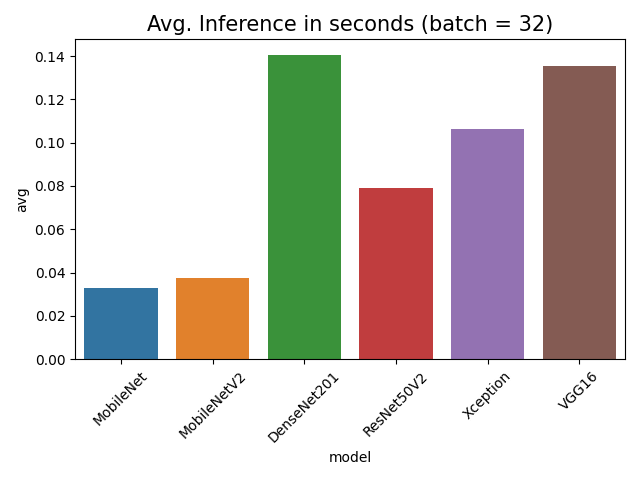
\includegraphics[width=\linewidth]{figures/inference.png}
\end{figure}

The results visualized in Fig. \ref{fig:result:inference} show that only \textit{MobileNet} and \textit{MobileNetV2} have near real-time capabilities. While a prediction time of 0.14 seconds (\textit{DenseNet201}, Fig. \ref{fig:result:inference}) does seem acceptable to the human eye, it translates to approx. 7 predictions per second. Given, that the human eye can detect meaning in images within 13ms\cite{Potter2014} (approx. 75 frames per second (fps)) and videos have a minimum framerate of 23.97 fps to appear smooth and fluent, 7 predictions (frames) per second will not lead to an acceptable user experience. Therefore only the \textit{MobileNet} and \textit{MobileNetV2} should be considered for real-time applications, as the inference time of 0.03 seconds leads to a framerate of approx. 33 fps.

\subsection{Translation Process}
<KEINE STATS, VERWEIS AUF BILD + IMPLEMENTIERUNG>
